\section{Evaluation}\label{sec:evaluation}

% This section shows benchmark designs and results of each papers' implementation by us.
% sand and fusionize attempt to solve similar problems -> same evaluation and
% comparison: latency benchmark aimed at measuring network overheads
% profaastinate is different -> own evaluation:
% all evaluations' results are discussed together in section
% \ref{sec:discussion}

This section provides an overview of our benchmark designs and the results of
our implementation for each paper. SAND and \textsc{Fusionize} attempt to solve
similar problems, hence they share the same evaluation and are directly compared
to each other. We primarily focus on the latency benchmark designed to measure
network overheads. On the other hand, \textsc{ProFaaStinate} is different from
the other approaches and therefore requires its own specific evaluation. The
outcomes of all these evaluations will be collectively discussed in Section
\ref{sec:discussion}.

\subsection{Fusionize and SAND}

% for fusionize and sand we designed a benchmark aimed at isolating the network
% overhead to simulate cascading cold starts and double billing. We chose method
% best showcases end to end latencies between faas functions we decided for
% synthetic base load to investigate system's performance under maximum stress.

% To showcase maximum latency, we designed two tasks, shown in Figure X,
% \emph{interface} task and \emph{counter} task. The counter Task receives a
% number and returns the number, incremented by one. The interface task receives
% a \emph{destination} number by the user and invokes the counter task, starting
% with the number zero. The result of the counter task is then used to invoke
% the counter task again until the destination number is reached.

% This proposed load generator is unconventional, as it resides within the
% system under test. However, this design allows for function invocation within
% the platfrom and most importantly \emph{between} functions. To start the
% benchmark, only the interface task needs to be invoked with destination
% number and latency between invocation and result is to measured.

\subsubsection{Experiment Setup}
\label{subsubsec:evaluation:fusionize_and_sand:experiment_setup}

For \textsc{Fusionize} and SAND, we have constructed a benchmark with the
intention of isolating networking overhead. This is designed to simulate scenarios
involving cascading cold starts and double billing. We made this decision based
on our belief that this approach most effectively displays the end-to-end
latencies that can occur between FaaS functions. We chose to employ a synthetic
base load for our testing in order to examine the system's performance under
maximum stress.

In order to illustrate the maximum latency, we devised two tasks. These tasks,
which can be seen in Figure \ref{fig:bench}, are known as the \emph{interface}
and \emph{counter} tasks. The objective of the counter task is to receive a
number and return the same number after it has been increased by one. The
interface task works by accepting a \emph{destination} number supplied by the
user, then invoking the counter task, beginning with the number zero. Following
this, the result of the counter task is used to again invoke the counter task,
repeating until the destination number is reached.

Our proposed load generator has an unconventional design, as it resides within
the system under test (SUT). However, this design allows function invocation
within the platform, and, even more crucially, between functions. This is
important, as both Fusionize and SAND are revolving around the communication
between FaaS functions. To initiate the benchmark, only the interface task needs
to be invoked with the destination number. The latency between the invocation
and result must then be measured.

% - In a production setting, Nuclio is run in k8s cluster
% - We configured deployment of our approaches for k8s
% - For our benchmarks we deployed our system in local Minikube cluster

In a production environment, Nuclio operates within a k8s cluster. We have
successfully configured the deployment of our approaches for operation within
the k8s environments. For benchmarking purposes, we deployed our system within a
local Minikube\footnote{\url{https://minikube.sigs.k8s.io/}} cluster.

\begin{figure}
    \centering
    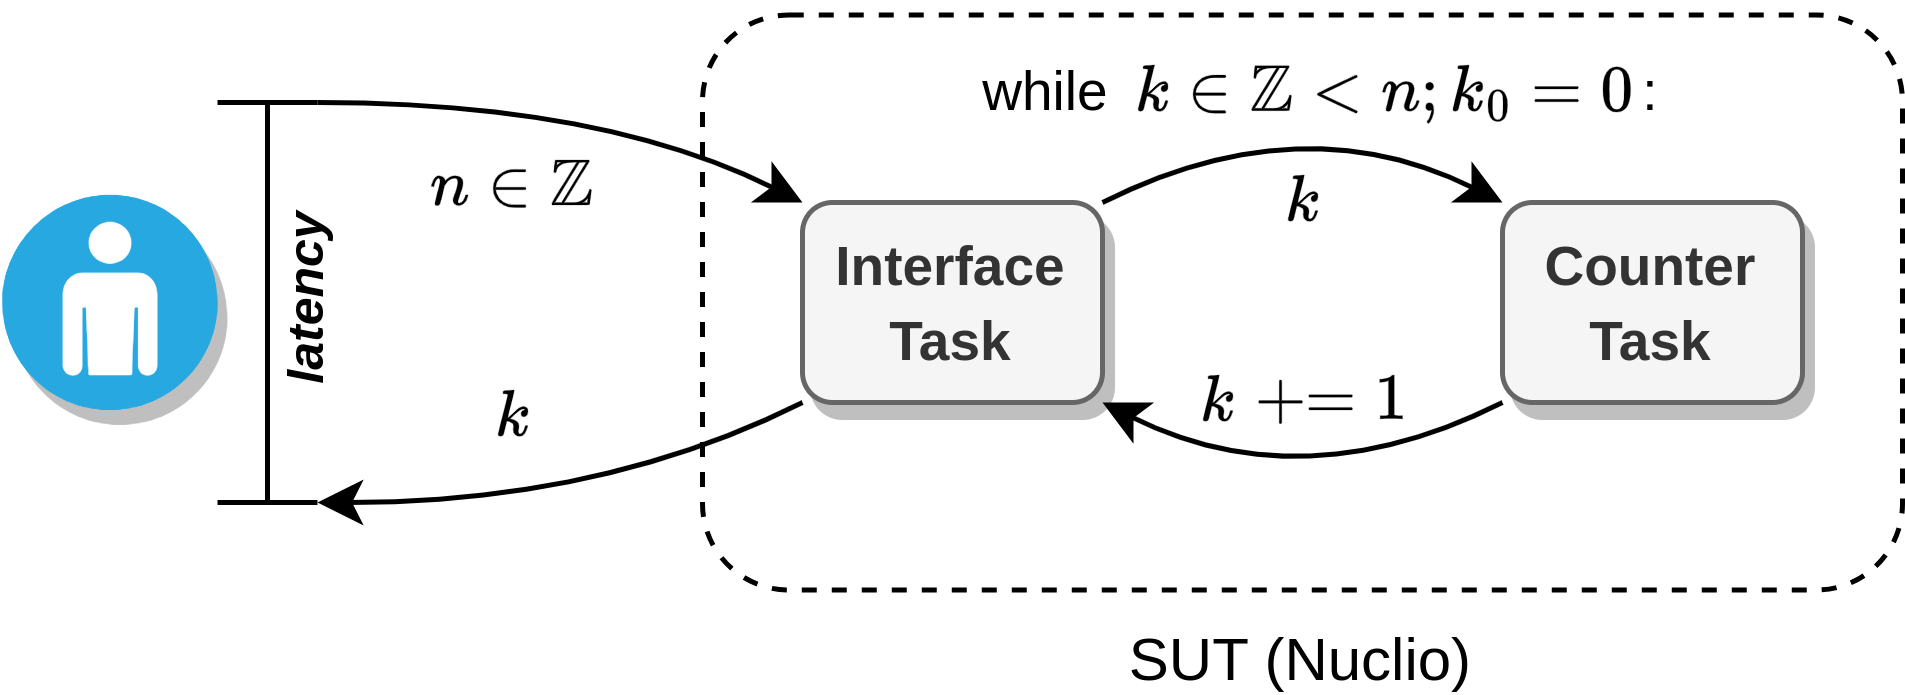
\includegraphics[width=\linewidth]{figures/bench}
    \caption{
        The Counter Task increments a given number by one. The Interface Task
        receives a target number from the user and repeatedly invokes the
        Counter Task, starting at zero, until the target number is achieved. The
        Interface Task then returns this number to the user upon completion of
        the benchmark run. This allows the user to measure the total end-to-end
        latency.
    }
    \label{fig:bench}
\end{figure}

\subsubsection{Results}
\label{subsubsec:evaluation:fusionize_and_sand:results}

\begin{figure}
    \centering
    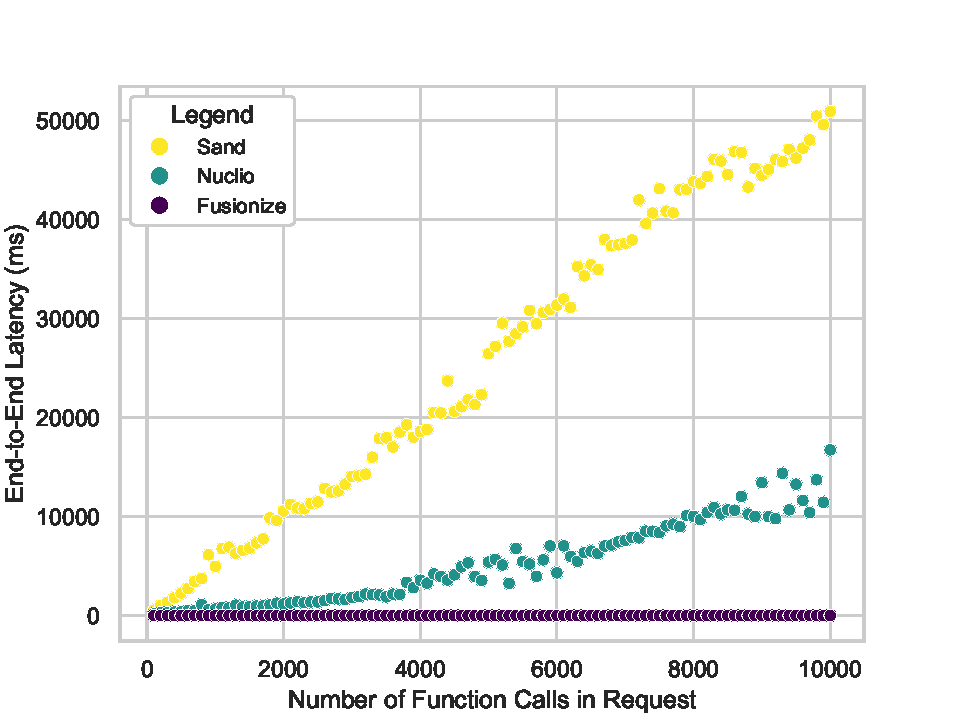
\includegraphics[width=\linewidth]{figures/latency_sand_fusionize}
    \caption{
        Results of our benchmark outlined in Figure \ref{fig:bench}. Our SAND
        implementation increases linearly and significantly faster than vanilla
        Nuclio. Our \textsc{Fusionize} implementation appears to have nearly
        constant latency.
    }
    \label{fig:latency_sand_fusionize}
\end{figure}


In Figure \ref{fig:latency_sand_fusionize}, we can see the results of our
benchmark. The x-axis shows the number of function calls required the answer the
request, and the y-axis show the measured end-to-end latency. As the interaction
between functions increases, the end-to-end latency increases linearly for SAND.
With 10,000 function calls, the SUT takes approximately 50 seconds to answer the
request using our SAND implementation. For vanilla Nuclio, the latency caused by
the same request if significantly lower at below 20 seconds. The end-to-end
latency of vanilla Nuclio scales exponentially with increasing interaction
between functions. With Fusionize, the latency is very close to 0 throughout the
experiment.


\subsection{ProFaaStinate}
\label{sec:eval-profaastinate}
In this section, we aim to evaluate the implementation status of both our functional and non-functional requirements as outlined in Section \ref{sec:functional-req}. To provide context for this assessment, we first outline our experiment setup, including the end-to-end test, and then present the results of the experiment. Finally, we analyze how well our system adheres to the defined requirements based on the results.

\subsubsection{Experiment Setup}

It's worth noting that we were unable to test the Bulk Scheduler in any meaningful way, as Nuclio only provides the scale to zero feature to enterprise users. We can confidently say that we did everything possible to implement that feature on our own, including a consultation with a developer from Nuclio. To the disadvantage of our experiment, we could not activate this feature. And without it, the integration of a Bulk Scheduler doesn't really make sense, although it does work.

In concrete terms, we aimed to evaluate the performance of ProFaaStinate when the Idle and Deadline schedulers are enabled. To achieve this, we devised a benchmark that subjects Nuclio to high load scenarios with asynchronous calls. By default, these calls are executed immediately in Nuclio, but with the schedulers enabled, they should be distributed evenly over time. The benchmark strategy involved imposing a constant load on Nuclio with a baseline of calls, while gradually increasing the load at intervals. We used k6, a load testing tool, to orchestrate and execute the benchmark.
The benchmark, which comprised function calls tasked with calculating prime numbers as well as executing functions named "vanilla" and "second", aimed at inducing high CPU utilization and compelling ProFaaStinate to delay certain calls. This setup initiated the benchmark with a base load of 800 requests having the deadline set to 4000 seconds. Subsequently, the benchmark sent a total of 800 requests at intervals, with the deadline between 5 seconds and 4000 seconds.
To ensure thorough validation of the implementation, we established an evaluation backend. This backend serves to record all function calls in the form of logs, enabling detailed analysis of the runtime information. The recorded data includes the following key attributes:
\begin{itemize}
    \item Function name: Identifies the specific function being called.
    \item Scheduler name: Specifies the scheduler responsible for managing the function's execution.
    \item Asynchronous  Deadline (timestamp)
    \item Start of synchronization processing (timestamp)
    \item Start of execution of function (timestamp)
    \item End of execution of function (timestamp)
\end{itemize}
We evaluated the benchmark within a Docker environment, as the performance of the Minikube environment proved to be inadequate—further details on this issue will be provided later. The tests were conducted on a system with the following specifications:
\begin{itemize}
    \item OS: Linux Mint 21.2 Cinnamon
    \item CPU: Inte i9-9900K
    \item RAM: 32GB
    \item GPU: AMD 6900xt
\end{itemize}

\subsection{Results}
% comparision
If required, our logs can be accessed directly via the Github repository to check our results\footnote{\url{https://github.com/valentin-carl/nuclio/tree/mpga-eval/profaastinate/evaluation/data-analysis/logs}}. 
We start with a comparison of how synchronous tasks in Nuclio without ProFaaStinate differ from asynchronous tasks with ProFaaStinate. 

\begin{figure}
    \centering
    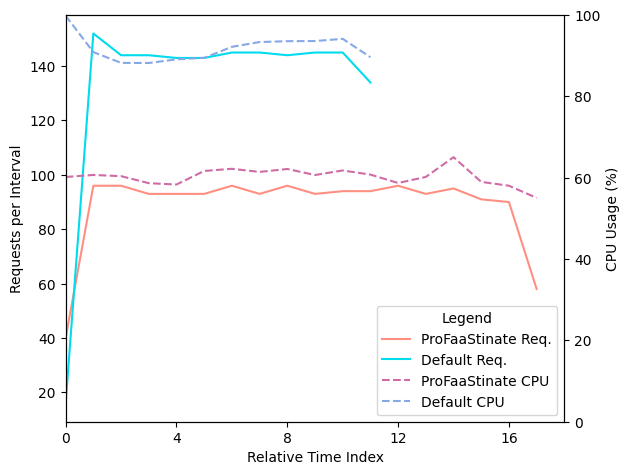
\includegraphics[width=\linewidth]{figures/profaastinate/results/line_chart.png}
    \caption{Default nuclio processing consumes higher peak CPU utilization and higher requests per interval, while ProFaaStinate processing requires a longer runtime.}
    \label{fig:metrics-comparision}
\end{figure}

In the graph \ref{fig:metrics-comparision}, the x-axis shows the relative time. This is a mapping of the timestamps of the default Nuclio and ProFaaStinate execution tests, which were executed one after the other and therefore had to be mapped to each other. The left y-axis describes the requests per interval, while the right y-axis shows the utilization of the system in relative time. There are 4 lines, with the red and orange ones referring to the ProFaaStinate calls and the bluish ones to the Default calls. 
It can be clearly seen that the Default lines are set higher than their respective counterparts. For example, the average CPU utilization in Default execution is around 90\%, while the utilization of the ProFaaStinate system is around 60\%. 
The situation is similar with the number of requests per interval in the standard setup, where around 140 are processed, while ProFaaStinate only processes 100. Default processing stops after about 10 time units, while ProFaaStinate processing continues until approximately 17. It should be noted that the level of CPU utilization in both modes is already relatively high at the beginning of the experiment and hardly decreases noticeably. It stands out that the standard processing is directly 100\% at the beginning.


\begin{figure}
    \centering
    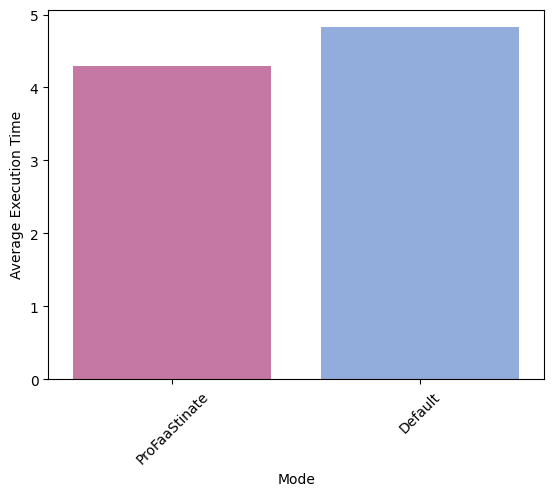
\includegraphics[width=\linewidth]{figures/profaastinate/results/execution_time_chart.png}
    \caption{ProFaaStinate Reduces Average Execution Time by 15\% Compared to Default Nuclio}
    \label{fig:execution-time-comparision}
\end{figure}

The diagram \ref{fig:execution-time-comparision} has the average execution time as the y-axis with values between 0 and 5. Meanwhile, the x-axis provides information about the mode, which is either ProFaaStinate or default Nuclio. While the average standard execution time is almost 5, with ProFaaStinate it is closer to 4.25. This means that function calls can be processed faster with ProFaaStinate than with default Nuclio.

\begin{figure}
    \centering
    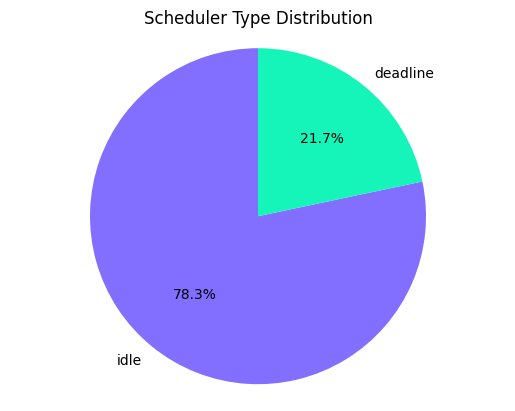
\includegraphics[width=\linewidth]{figures/profaastinate/results/pie_chart.png}
    \caption{
        Idle Scheduler Handles Majority of Function Invocations in ProFaaStinate
        %Results of the benchmark performed with ProFaaStinate implemented. It indicates the distribution between the Deadline Scheduler and the Idle Scheduler of processed entries. It shows that the Idle Scheduler processed the largest amount of function invocation requests.
    }
    \label{fig:scheduler-distribution}
\end{figure}
Having previously compared asynchronous and synchronous processing, we will now only focus on the insights of asynchronous processing.
Figure \ref{fig:scheduler-distribution} showcases the activity of the Idle and Deadline Scheduler during the benchmark with ProFaaStinate.  It indicates that the Idle Scheduler processed 78.3\% of the function invocation requests, and the Deadline Scheduler only processed 21.7\% of the function invocation requests. Consequently, the Idle Scheduler processed the largest number of requests.

\subsection*{Fullfillments of Functional Requirements}
The following section evaluates whether or not the functional requirements have been met. Relevant key figures from the test are used for this purpose. 
\begin{itemize}
    \item \textbf{Asynchronous function execution}: In our tests, all 1600 requests that were sent asynchronously to the Nuclio system triggered a callback on our evaluation backend. Since all requests arrived according to the protocols, every intermediate step, including the \nameref{sec:nexus-queue}, must function seamlessly. 
    Furthermore, we can observe in Figure \ref{fig:execution-time-comparision} that the execution time of requests, is slightly reduced, the reason for that is the CPU possible throtteling of the system, when operating at its processing limit. This effect could be particularly advantageous in environments in which synchronous and therefore time-critical requests also lie between the asynchronous requests. This is because, as explained in \nameref{sec:ProFaaStinate_Concept}, a calling component might wait for the response, hence latency plays a role. 
    This requirement is considered fulfilled.
    
    \item \textbf{Different Scheduler Types}: This requirement has been achieved by implementing the various scheduler types \nameref{sec:deadline-scheduler}, \nameref{sec:idle-scheduler} and \nameref{sec:bulk-scheduler}. Each scheduler type serves specific purposes and operates independently, ensuring that resources are optimally utilized and separation of concerns is respected. According to the logs and the benchmark (Figure \ref{fig:scheduler-distribution}), all tasks are executed within the deadline and both the idle and the Deadline Scheduler have processed function calls. We can therefore confirm that the simultaneous use of multiple schedulers is possible. However, the Deadline Scheduler only intervenes in an emergency to ensure timely processing.
    
    \item \textbf{Configuration Flexibility}: This requirement has also been met by offering both constructors as well as default factory constructors that enable smooth integration of components into the setup. In addition, we offer users the option of dynamically starting and stopping schedulers during runtime via a REST interface. The attributes of the Load Balancer can also be changed during runtime via REST, allowing the system to be fine-tuned to research requirements as required.
\end{itemize}

\subsection*{Fullfillments of Non-Functional Requirements}
After the functional requirements, the non-functional requirements must now be checked.
\begin{itemize}
    \item \textbf{Abstraction layer}: We have successfully implemented this requirement by integrating the entire logic of ProFaaStinate into our own package "Nexus". The Nexus package functions as a stand-alone unit and is only activated via a dashboard link and the deadline header. This ensures a clear separation between the integrated logic and the external components.
    \item \textbf{Modular extensible architecture}: In building our modular and extensible architecture, we applied key design patterns. We used the factory pattern to simplify component integration by providing default values where needed. Additionally, the composite pattern facilitated component structuring, particularly evident in models like the \nameref{sec:bulk-scheduler} and base scheduler. For complex deployment processes, we implemented the facade pattern with the \nameref{sec:elastic-deploy}, offering simplified interface for the schedulers to attach to instead of directly assigning the docker or kube environment. 
    In addition, the composite creation pattern was used to build new schedulers, see \nameref{sec:base-scheduler}. This system is based on the Load Balancer, which proves to be effective in its implementation. For the experiment, the described default values from the section \ref{sec:load-balancer} were used, where the Load Balancer should only allow new requests up to 60\% load. This does not work for a short time, as the load is closer to 70\% at time unit 14; this is corrected again directly in the next interval. This means that the scheduler creator does not have to worry about his scheduler overloading the system.
    This requirement is considered fulfilled.

    \item \textbf{Documentation}: In terms of documentation, our final submission included detailed README files covering all areas, as well as separate guides for deploying the software to Kubernetes and Docker environments. In addition, in-code documentation was provided for all Golang files to improve developers' understanding of the codebase. Futhermore, 9 UML diagrams have been created to illustrate workflow scenarios and component relationships within the system. With these documentation resources, users should be able to effectively understand the software and its architecture, fulfilling this requirement

    \item \textbf{Unit tests}
    Unfortunately, the targeted percentage of 75\% could not be achieved and in the end we only achieved a test coverage rate of 62.3\%. Factors that contributed to this shortfall include a lack of time, the complexity of the code base and a lack of experience in the project lanaguage Golang. However this deviation is probably still enough in a test project that primarily serves research purposes, but it remains the case that we were unable to fulfill this point.
\end{itemize}